\let\negmedspace\undefined
\let\negthickspace\undefined
\documentclass[journal,12pt,onecolumn]{IEEEtran}
\usepackage{cite}
\usepackage{amsmath,amssymb,amsfonts,amsthm}
\usepackage{algorithmic}
\usepackage{graphicx}
\graphicspath{{./figs/}}
\usepackage{textcomp}
\usepackage{xcolor}
\usepackage{txfonts}
\usepackage{listings}
\usepackage{enumitem}
\usepackage{mathtools}
\usepackage{gensymb}
\usepackage{comment}
\usepackage{caption}
\usepackage[breaklinks=true]{hyperref}
\usepackage{tkz-euclide} 
\usepackage{listings}
\usepackage{gvv}                                        
%\def\inputGnumericTable{}                                 
\usepackage[latin1]{inputenc}     
\usepackage{xparse}
\usepackage{color}                                            
\usepackage{array}                                            
\usepackage{longtable}                                       
\usepackage{calc}                                             
\usepackage{multirow}
\usepackage{multicol}
\usepackage{hhline}                                           
\usepackage{ifthen}                                           
\usepackage{lscape}
\usepackage{tabularx}
\usepackage{array}
\usepackage{float}
%\newtheorem{theorem}{Theorem}[section]
%\newtheorem{theorem}{Theorem}[section]
%\newtheorem{problem}{Problem}
%\newtheorem{proposition}{Proposition}[section]
%\newtheorem{lemma}{Lemma}[section]
%\newtheorem{corollary}[theorem]{Corollary}
%\newtheorem{example}{Example}[section]
%\newtheorem{definition}[problem]{Definition}

\begin{document}

\begin{center}
\textbf{\Large XL: Life Sciences} \\
\textbf{\large AI25BTECH11001 - Abhisek Mohapatra} \\
\textbf{H: Chemistry (Compulsory)}
\textbf{Q.1-Q.6 carry one mark each.}
\end{center}

\begin{enumerate}
    \item On the basis of VSEPR theory, the molecule which has a linear structure is 
    \begin{multicols}{4}
        \begin{enumerate}
            \item $SO_{2}$ 
            \item $N_{2}O$ 
            \item $Cl_{2}O$ 
            \item $NO_{2}$ 
        \end{enumerate}
    \end{multicols}
	    \hfill \textbf{GATE XL 2007}%TODO

    \item The geometries of $[NiCl_{4}]^{2-}$ and $[PdCl_{4}]^{2-}$ respectively are 
        \begin{enumerate}
	\item Tetrahedral and square planar
            \item Both tetrahedral
            \item Both square planar
            \item Square planar and tetrahedral
        \end{enumerate}
	    \hfill \textbf{GATE XL 2007}%TODO

    \item The ionization energy of hydrogen atom in ground state is 13.6 eV. The ionization energy of $Li^{2+}$ in ground state would be 
    \begin{multicols}{4}
        \begin{enumerate}
            \item 1.51 eV
            \item 4.53 eV
            \item 40.8 eV
            \item 122.4 eV
        \end{enumerate}
    \end{multicols}
	    \hfill \textbf{GATE XL 2007}%TODO

    \item The half-life of $^{14}C$ is 5730 years. An old sample of wood contains 25\% of $^{14}C$ would be found in a current living tree. The age of the sample of wood would be 
    \begin{multicols}{4}
        \begin{enumerate}
            \item 1432 years
            \item 2865 years
            \item 5730 years
            \item 11460 years
        \end{enumerate}
    \end{multicols}
	    \hfill \textbf{GATE XL 2007}%TODO

    \item The product 'P' formed in the following reaction is 
\begin{figure}[h!]
	\centering
	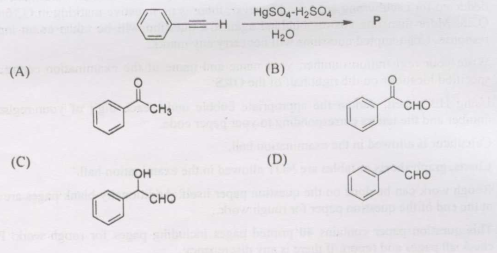
\includegraphics[width=10cm]{5}
	\caption*{}
	\label{fig:Q5}
	\end{figure}



	    \hfill \textbf{GATE XL 2007}%TODO

    \item The order of reactivity of the following aldehydes with a nucleophile is %image 
    
\begin{figure}[h!]
	\centering
	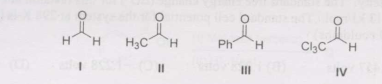
\includegraphics[width=10cm]{6}
	\caption*{}
	\label{fig:Q6}
	\end{figure}
    \begin{multicols}{2}
        \begin{enumerate}
            \item I $>$ II $>$ III $>$ IV
            \item IV $>$ II $>$ III $>$ I
            \item IV $>$ III $>$ II $>$ I
            \item I $>$ IV $>$ II $>$ III
        \end{enumerate}
    \end{multicols}
	    \hfill \textbf{GATE XL 2007}
\end{enumerate}

\subsection*{Q.7-Q.24 carry two marks each.}

\begin{enumerate}[resume]
    \item In the nuclear reaction of $^{235}_{92}U$ with a neutron, two elements, Kr and 'Y', are formed along with three neutrons. 
    \[^{235}_{92}U + ^{1}_{0}n \rightarrow ^{92}_{36}\text{Kr} + 3 ^{1}_{0}n + \text{Y}\]
    The element 'Y' is
    \begin{multicols}{4}
        \begin{enumerate} 
            \item $^{142}_{56}\text{Ba}$
            \item $^{142}_{55}\text{Cs}$
            \item $^{142}_{54}\text{Xe}$
            \item $^{142}_{53}\text{I}$
        \end{enumerate}
    \end{multicols}
	    \hfill \textbf{GATE XL 2007}

    \item Which of the following statements is true about diatomic species $\text{He}_{2}$ and $\text{He}_{2}^{+}$? 
        \begin{enumerate} 
            \item $\text{He}_{2}$ is stable AND $\text{He}_{2}^{+}$ is stable
            \item $\text{He}_{2}$ is stable AND $\text{He}_{2}^{+}$ is unstable
            \item $\text{He}_{2}$ is unstable AND $\text{He}_{2}^{+}$ is stable
            \item $\text{He}_{2}$ is unstable AND $\text{He}_{2}^{+}$ is unstable
        \end{enumerate}
    
	    \hfill \textbf{GATE XL 2007}

    \item For the reaction A $\rightleftharpoons$ B, the activation energy for the forward reaction is 123 kJ/mol. The activation energy for the reverse reaction is 140 kJ/mol. The enthalpy change for the forward reaction is 
    \begin{multicols}{4}
        \begin{enumerate} 
            \item 263 kJ/mol
            \item -263 kJ/mol
            \item 17 kJ/mol
            \item -17 kJ/mol
        \end{enumerate}
    \end{multicols}

	    \hfill \textbf{GATE XL 2007}
    \item The acid dissociation constant of a weak acid HA is $10^{-5}$. A 0.20 M solution of the acid HA also contains 0.10 M of salt $MA_{2}$. The pH of the solution is 
    \begin{multicols}{4}
        \begin{enumerate} 
            \item 0.69
            \item 1.0
            \item 2.85
            \item 5.0
        \end{enumerate}
    \end{multicols}

	    \hfill \textbf{GATE XL 2007}
    \item The attractive part of the van der Waals interaction, $-B/r^{6}$, where B is a positive coefficient and r is the distance between the molecules, is governed by 
        \begin{enumerate} 
            \item dipole-dipole interaction
            \item charge-dipole interaction
            \item induced dipole-induced dipole interaction
            \item dipole-induced dipole interaction
        \end{enumerate}
	    \hfill \textbf{GATE XL 2007}

    \item A fuel cell is based on the idea of the reaction $H_{2}(g)+\frac{1}{2}O_{2}(g)\rightarrow H_{2}O(l)$ generating electricity. The standard free energy change $(\Delta G^{\circ})$ for this reaction at 298 K is -237.13 kJ/mol. The standard cell potential for the system at 298 K is (1 Faraday = 96500 coulombs) 
    \begin{multicols}{4}
        \begin{enumerate} 
            \item 2.457 volts
            \item 1.228 volts
            \item -1.228 volts
            \item -2.457 volts
        \end{enumerate}
    \end{multicols}

	    \hfill \textbf{GATE XL 2007}
    \item The electron-deficient molecule is 
    \begin{multicols}{4}
        \begin{enumerate} 
            \item $N_{2}H_{4}$
            \item $C_{2}H_{6}$
            \item $B_{2}H_{6}$
            \item $O_{2}H_{2}$
        \end{enumerate}
    \end{multicols}
	    \hfill \textbf{GATE XL 2007}

    \item The complex with crystal field stabilization energy (CFSE) of -0.4 $\Delta_{t}$ is 
    \begin{multicols}{4}
        \begin{enumerate} 
            \item $[TiCl_{4}]$
            \item $[MnCl_{4}]^{2-}$
            \item $[CoCl_{4}]^{2-}$
            \item $[CuCl_{4}]^{2-}$
        \end{enumerate}
    \end{multicols}
	    \hfill \textbf{GATE XL 2007}

    \item The most stable geometry of $BrF_{5}$ is \%image \hfill \textbf{GATE XL 2007}
    \begin{figure}[h!]
	\centering
	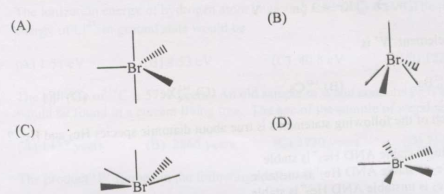
\includegraphics[width=10cm]{15}
	\caption*{}
	\label{fig:Q15}
	\end{figure} 
\item The species having three unpaired electrons and tetrahedral geometry is 
    \begin{multicols}{4}
        \begin{enumerate} 
            \item $[Co(CN)_{6}]^{4-}$
            \item $[CoCl_{4}]^{2-}$
            \item $[Ni(CN)_{4}]^{2-}$
            \item $[NiCl_{4}]^{2-}$
        \end{enumerate}\hfill{\textbf{GATE XL 2007}}
    \end{multicols}
	    \hfill \textbf{GATE XL 2007}

    \item The correct arrangement of group 13 elements in terms of increasing average M-Cl bond energy in $MCl_{3}$ compounds is 
        \begin{enumerate} 
            \item $Al>Ga>In>TI$
            \item $T1>In>Ga>Al$
            \item $Al>Ga>TI>In$
            \item $Ga>In>TI>Al$
        \end{enumerate}

	    \hfill \textbf{GATE XL 2007}
    \item Which of the following olefins leads to a racemic mixture of the diol product upon cis-dihydroxylation? %image \hfill \textbf{GATE XL 2007}
    \begin{figure}[h!]
	\centering
	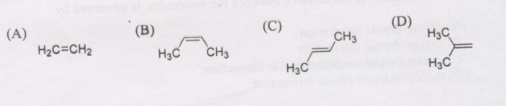
\includegraphics[width=10cm]{18}
	\caption*{}
	\label{fig:Q18}
	\end{figure} 
	    \hfill \textbf{GATE XL 2007}
\clearpage
    \item The major product 'Q' formed in the following reaction is%image
    \begin{figure}[h!]
	\centering
	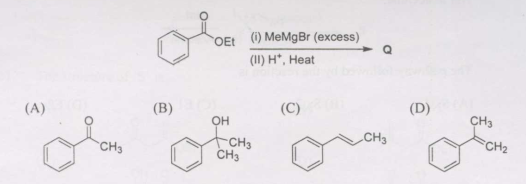
\includegraphics[width=10cm]{19}
	\caption*{}
	\label{fig:Q19}
	\end{figure} 
	    \hfill \textbf{GATE XL 2007}

    \item The most stable conformation of cis-1-tert-butyl-4-methylcyclohexane is 
    \begin{figure}[h!]
	\centering
	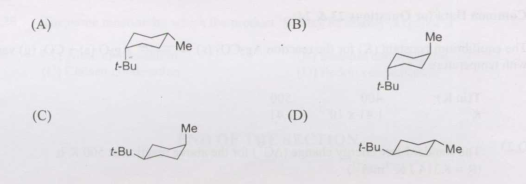
\includegraphics[width=10cm]{20}
	\caption*{}
	\label{fig:Q20}
	\end{figure} 
	    \hfill \textbf{GATE XL 2007}

    \item The major product 'R' formed in the following reaction sequence is \%image 
    \begin{figure}[h!]
	\centering
	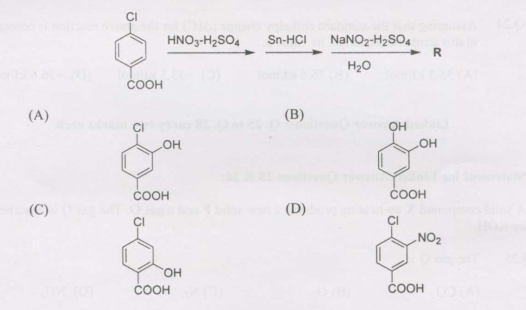
\includegraphics[width=10cm]{21}
	\caption*{}
	\label{fig:Q21}
	\end{figure} 
	    \hfill \textbf{GATE XL 2007}

    \item The following optically active compound undergoes racemization upon reaction with NaI in acetone. 
    \begin{figure}[h!]
	\centering
	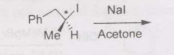
\includegraphics[width=10cm]{22}
	\caption*{}
	\label{fig:Q22}
	\end{figure} 
	    \hfill \textbf{GATE XL 2007}

    \item The pathway followed by the reaction is
	    
    \begin{multicols}{4}
        \begin{enumerate} 
            \item $S_{N}1$
            \item $S_{N}2$
            \item E$_1$
            \item E2$_2$
        \end{enumerate}
    \end{multicols}
\end{enumerate}

\textbf{Common Data Questions}
\noindent\textbf{Common Data for Questions 23 \& 24:}
The equilibrium constant (K) for the reaction $Ag_{2}CO_{3} (s) \rightleftharpoons Ag_{2}O (s) + CO_{2} (g)$ varies with temperature T as

%\begin{tabular}{}
%     T (in K) &  K \\
%     400 &  $1.41 \times 10^{-2}$ \\
%     500 &  1.41 \\
%\end{tabular}

\begin{enumerate}
    \item The standard free energy change $(\Delta G^{0})$ for the above reaction at 500 K is ($R = 8.314 \text{ J } K^{-1} \text{mol}^{-1}$) 
    \begin{multicols}{4}
        \begin{enumerate} 
            \item $-0.62$ kJ/mol
            \item $-1.43$ kJ/mol
            \item $0.62$ kJ/mol
            \item $1.43$ kJ/mol
        \end{enumerate}
    \end{multicols}
	    \hfill \textbf{GATE XL 2007}

    \item Assuming that the standard enthalpy change $(\Delta H^{\circ})$ for the above reaction is constant in this temperature range, its value is 
    \begin{multicols}{4}
        \begin{enumerate} 
            \item $33.3$ kJ/mol
            \item $76.6$ kJ/mol
            \item $-33.3$ kJ/mol
            \item $-76.6$ kJ/mol
        \end{enumerate}
    \end{multicols}
	    \hfill \textbf{GATE XL 2007}


\textbf{Linked Answer Questions: Q. 25 to Q. 28 carry two marks each.}
\noindent\textbf{Statement for Linked Answer Questions 25 \& 26:}
A solid compound X on heating produces a new solid P and a gas Q. The gas Q is absorbed by KOH.


    \item The gas Q is 
    \begin{multicols}{4}
        \begin{enumerate} 
            \item $CO_{2}$
            \item $O_{2}$
            \item $N_{2}$
            \item $NH_{3}$
        \end{enumerate}
    \end{multicols}
	    \hfill \textbf{GATE XL 2007}

    \item The reaction between P and water forms a new compound R. Compound R gives bleaching powder on reaction with $Cl_{2}$. The compound X is 
    \begin{multicols}{4}
        \begin{enumerate} 
            \item $NH_{4}NO_{2}$
            \item $KClO_{3}$
            \item $CaCO_{3}$
            \item $CuFeS_{2}$
        \end{enumerate}
    \end{multicols}
	    \hfill \textbf{GATE XL 2007}

\textbf{Statement for Linked Answer Questions 27 \& 28:}
    \item The structure of 'S' is %image 
    \begin{figure}[h!]
	\centering
	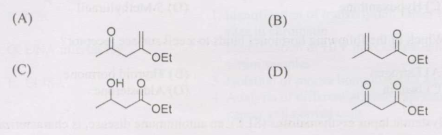
\includegraphics[width=10cm]{27}
	\caption*{}
	\label{fig:Q27}
	\end{figure} 
	    \hfill \textbf{GATE XL 2007}

    \item The name reaction by which the product 'S' may be readily prepared is 
    \begin{multicols}{2}
        \begin{enumerate} 
            \item Aldol condensation
            \item Benzoin condensation
            \item Claisen condensation
            \item Perkin condensation
        \end{enumerate}
    \end{multicols}
\end{enumerate}
\begin{center}
\textbf{END OF THE SECTION}
\end{center}

\newpage

\section*{I: Biochemistry}
\subsection*{Q.1-Q.6 carry one mark each.}

\begin{enumerate}
    \item Deamination of cytosine produces 
    \begin{multicols}{2}
        \begin{enumerate} 
            \item Uracil
            \item Pseudouracil
            \item Hypoxanthine
            \item 5-Methyluracil
        \end{enumerate}
    \end{multicols}
	    \hfill \textbf{GATE XL 2007}

    \item Which of the following hormones binds to a cell surface receptor? 
    \begin{multicols}{2}
        \begin{enumerate} 
            \item Estrogen
            \item Thyroid hormone
            \item Insulin
            \item Aldosterone
        \end{enumerate}
    \end{multicols}
	    \hfill \textbf{GATE XL 2007}

    \item Systemic lupus erythematosus (SLE), an autoimmune disease, is characterized by the presence of 
    \begin{multicols}{2}
        \begin{enumerate} 
            \item Anti-DNA antibodies
            \item Anti-thyroglobulin antibodies
            \item Anti-insulin antibodies
            \item Anti-collagen antibodies
        \end{enumerate}
    \end{multicols}
	    \hfill \textbf{GATE XL 2007}

    \item Optical density of 1 means 
        \begin{enumerate} 
            \item 1\% of the incident light is absorbed
            \item 1\% of the incident light is transmitted
            \item 90\% of the incident light is absorbed
            \item 90\% of the incident light is transmitted
        \end{enumerate}
	    \hfill \textbf{GATE XL 2007}

    \item One of the carbon atoms of a glucose molecule is $[^{14}C]$-labeled. If $^{14}CO_{2}$ is released during the conversion of pyruvate to acetyl coenzyme-A, which carbon atom of glucose was radiolabeled? 
        \begin{enumerate} 
            \item C3 but not C4
            \item C3 or C4
            \item C1 or C6
            \item C1 but not C6
        \end{enumerate}
	    \hfill \textbf{GATE XL 2007}

    \item When yeast cells are shifted from a medium containing glycerol to glucose, an increase in the transcription of four genes involved in glucose metabolism was reported. Which of the following would be the most appropriate technique to demonstrate increased transcription of these genes? 
    \begin{multicols}{2}
        \begin{enumerate} 
            \item Southern hybridization
            \item Northern hybridization
            \item Western hybridization
            \item Fluorescence in situ hybridization
        \end{enumerate}
    \end{multicols}
	    \hfill \textbf{GATE XL 2007}

\subsection*{Q.7-Q.24 carry two marks each.}

    \item A mixture containing protein-1, -2, -3, -4, and -5 with molecular weights 5,000, 10,000, 25,000, 65,000, and 100,000, respectively, were separated on a Sephadex G-50 column. The order of elution of these proteins from the column will be 
        \begin{enumerate} 
            \item Protein-1, protein-2, protein-3, protein-4, and protein-5
            \item Protein-5, protein-4, protein-3, protein-2, and protein-1
            \item Protein-1, -2, and -3 elute first, followed by protein-5 and -4
            \item Protein-4 and -5 elute first, followed by protein-3, -2, and -1
        \end{enumerate}

	    \hfill \textbf{GATE XL 2007}
    \item The maximum number of hydrogen bonds that a molecule of water can form is 
    \begin{multicols}{4}
        \begin{enumerate} 
            \item 1
            \item 2
            \item 3
            \item 4
        \end{enumerate}
    \end{multicols}
	    \hfill \textbf{GATE XL 2007}

    \item Match the techniques mentioned in Column A with their applications given in Column B. 
    

	    \begin{tabularx}{\textwidth}{@{}lX@{}}
        \textbf{A} & \textbf{B} \\
        P. PCR & 1. Identification of transcription factor binding sites in chromatin \\
        Q. DNA microarray & 2. Identification of HIV infected patients using serum samples \\
        R. ELISA & 3. Isolation of mouse homologue of a yeast gene \\
        & 4. Analysis of differential gene expression in cancer and normal cells \\
    \end{tabularx}
        \begin{enumerate} 
            \item P-4, Q-1, R-3
            \item P-3, Q-4, R-2
            \item P-4, Q-1, R-2
            \item P-3, Q-2, R-1
        \end{enumerate}
	    \hfill \textbf{GATE XL 2007}

    \item A nonsense mutation in the gene encoding protein X leading to the synthesis of a truncated protein results in a slow growing strain. Mutagenesis of this strain towards the isolation of extragenic suppressors led to the isolation of a strain which grew normally and synthesized the full-length protein X. The extragenic suppressor is likely to be a gene coding for 
    \begin{multicols}{2}
        \begin{enumerate} 
            \item rRNA
            \item RNA polymerase
            \item tRNA
            \item Ribosomal protein
        \end{enumerate}
    \end{multicols}
	    \hfill \textbf{GATE XL 2007}

    \item The total radioactivity in 1 ml solution containing 0.25 mg of glycine is 1 mCi. The specific activity (mCi/millimole) of radiolabeled glycine will be
    \begin{multicols}{4}
        \begin{enumerate} 
            \item 300
            \item 18.75
            \item 3000
            \item 1875
        \end{enumerate}
    \end{multicols}
	    \hfill \textbf{GATE XL 2007}

    \item Ten grams of butter was saponified. The non-saponifiable fraction was extracted into 25 ml of chloroform. The absorbance of this solution in a 1 cm cuvette is 0.53 at 328 nm. If the extinction coefficient ($a_{1\%}$) of vitamin A at this wavelength is 1550, calculate the amount of vitamin A present. 
    \begin{multicols}{2}
        \begin{enumerate} 
            \item $3.419 \times 10^{-3}$ g/100 ml
            \item $3.419 \times 10^{-6}$ g/100 ml
            \item $3.419 \times 10^{-5}$ g/100 ml
            \item $3.419 \times 10^{-4}$ g/100 ml
        \end{enumerate}
    \end{multicols}
    
	    \hfill \textbf{GATE XL 2007}
    \item Folate derivatives are required for the synthesis of which deoxynucleotides? 
    \begin{multicols}{2}
        \begin{enumerate} 
            \item Adenylate and guanylate
            \item Cytidylate and thymidylate
            \item Adenylate, guanylate and thymidylate
            \item Adenylate, guanylate and cytidylate
        \end{enumerate}
    \end{multicols}

	    \hfill \textbf{GATE XL 2007}

    \item Cytochrome C reductase, also called as Complex III or cytochrome $bc_{1}$ complex, localized on the inner mitochondrial membrane receives electrons from ubiquinol and donates to cytochrome C. In one cycle, 
        \begin{enumerate} 
            \item Two cytochrome C molecules are reduced
            \item One ubiquinol is oxidized
            \item Two ubiquinols are oxidized and one ubiquinone is reduced
            \item One cytochrome C is reduced
        \end{enumerate}
    
	    \hfill \textbf{GATE XL 2007}
    \item Match the biological functions mentioned in Column A with the enzymes given in Column B. 
    \begin{tabularx}{\textwidth}{@{}lX@{}}
        \textbf{A} & \textbf{B} \\
        P) Diacylglycerol synthesis & (1) Protein kinase A \\
        Q) CREB phosphorylation & (2) Ras \\
        R) GTP hydrolysis & (3) Phospholipase C \\
        & (4) Phospholipase D \\
        & (5) Protein kinase G \\
    \end{tabularx}
        \begin{enumerate} 
            \item P-3, Q-1, R-5
            \item P-4, Q-1, R-2
            \item P-3, Q-1, R-2
            \item P-3, Q-5, R-2
        \end{enumerate}
	    \hfill \textbf{GATE XL 2007}
    
    \item How does haemoglobin carry carbon dioxide generated in tissues back to the lungs? 
        \begin{enumerate} 
            \item By coordination with heme
            \item By forming N-terminal carbamate
            \item By forming C-terminal carbamate
            \item By linking to the epsilon-amino group of lysine
        \end{enumerate}

	    \hfill \textbf{GATE XL 2007}
    \item Which of the following enzyme activities can be detected in the supernatant obtained by centrifugation of liver homogenate at 100,000 g for 1 hr at 4$^{\circ}$C? 
        \begin{enumerate} 
            \item Succinate dehydrogenase
            \item Glyceraldehyde 3-phosphate dehydrogenase
            \item Glycogen synthetase
            \item Aconitase
        \end{enumerate}
    
	    \hfill \textbf{GATE XL 2007}
    \item Which of the following statements about the enzyme complexes of the electron transport system is 'correct? 
        \begin{enumerate} 
            \item They interact with one another via mobile electron carriers
            \item They are located in the mitochondrial matrix
            \item They can not be separated from one another in a functional form
            \item They all have cytochromes
        \end{enumerate}
	    \hfill \textbf{GATE XL 2007}
\end{enumerate}
\begin{center}
\textbf{END OF THE SECTION}
\end{center}
%WAIT A MINUTE
\newpage

\section*{J: Biotechnology}
\subsection*{Q.1-Q.6 carry one mark each.}
\begin{enumerate}
    \item The specific growth rate (1) of a microorganism in death phase is
	    \begin{multicols}{2}
        \begin{enumerate} 
            \item 0
            \item max
            \item less than zero
            \item greater than zero
        \end{enumerate}
    \end{multicols}

	    \hfill \textbf{GATE XL 2007}
    \item Which of the following reagents is used for harvesting anchorage-dependent animal cells from culture vessels?
    \begin{multicols}{2}
        \begin{enumerate} 
            \item Trypsin/Collagenasem
            \item Trypsin/Collagen
            \item Collagen/Fibronectin
            \item DMSO
        \end{enumerate}
    \end{multicols}

	    \hfill \textbf{GATE XL 2007}
    \item Protein binding regions of DNA are identified by one of the following techniques

    \begin{multicols}{2}
        \begin{enumerate} 
            \item finger printing 
            \item foot printing
            \item southern blotting 
            \item western blotting
        \end{enumerate}
    \end{multicols}

	    \hfill \textbf{GATE XL 2007}
    \item Plant secondary metabolites
    \begin{multicols}{2}
        \begin{enumerate} 
            \item help to increase the growth rate of plant
            \item help in plant reproduction processes
            \item provide defense mechanisms against microbial attack
            \item make the plant susceptible to unfavorable conditions		    

	\end{enumerate}
    \end{multicols}
	    \hfill \textbf{GATE XL 2007}

    \item Si RNA(s) interfere at
    \begin{multicols}{2}
        \begin{enumerate} 
            \item transcriptional level 
            \item post-transcriptional level
            \item DNA replication level
            \item translational level
        \end{enumerate}
    \end{multicols}
	    \hfill \textbf{GATE XL 2007}

    \item Presence of CX2.4CXoXgHX3H sequence in a protein suggest that it is
	    \begin{multicols}{2}
        \begin{enumerate} 
            \item a protein kinase 
	    \item GTP binding proteinm
            \item zine finger protein 
            \item lipase
        \end{enumerate}
    \end{multicols}
	    \hfill \textbf{GATE XL 2007}
\subsection*{Q.7-Q.28 carry two marks each.}
    \item A protein binds to phosphocellulose column at pH 7.0 and elutes at pH 8.0. If the protein has to be further purified on a DEAE Sephacel column, the binding buffer should have a pH of
    \begin{enumerate}
        \item 5
        \item 6
        \item 7
        \item 8
    \end{enumerate}

	    \hfill \textbf{GATE XL 2007}
    \item Oils rich in PUFA are NOT desirable for bio-diesel production because
    \begin{enumerate}
        \item they form epoxides in presence of oxygen
        \item they do not form epoxides in presence of oxygen
        \item they have high ignition temperature
        \item they solidify at low temperature
    \end{enumerate}
	    \hfill \textbf{GATE XL 2007}

    \item Gynogenesis is a process of development of haploid plants
    \begin{enumerate}
        \item from a fertilized cell of female gametophyte
        \item from an unfertilized cell of female gametophyte
        \item from isolated pollen grains
        \item by selective elimination of chromosomes following distant hybridization
    \end{enumerate}
	    \hfill \textbf{GATE XL 2007}

    \item Match items in group 1 with correct examples from those in group 2
    
    

    \begin{tabularx}{\textwidth}{@{}lX@{}}
	    \textbf{Group 1} & \textbf{Group 2}\\
	     Catabolic product & 1. Griseofulvin\\
	     Bioconversion & 2. Bakers yeast\\
		    Biosynthetic product & 3. 6- Aminopenicillanic acid\\
	     Cell mass & 4. Ethanol\\
    \end{tabularx}
    \begin{enumerate}
        \item P-4, Q-3, R-2, S-1
        \item P-3, Q-4, R-1, S-2
        \item P-4, Q-3, R-1, S-2
        \item P-1, Q-4, R-3, S-2
    \end{enumerate}
	    \hfill \textbf{GATE XL 2007}

    \item A bioremedial solution to reduce oxides of nitrogen and carbon in flue gases is to integrate flue gas emission to
    \begin{enumerate}
        \item micro-algal culture
        \item fish culture
        \item mushroom culture
        \item seri culture
    \end{enumerate}
	    \hfill \textbf{GATE XL 2007}

    \item The respiratory coefficient for the reaction $a CH_mO_n + b O_2 + c NH_3 \rightarrow d C H_p O_q N_r + e H_2O + f CO_2$ is defined as
	    \begin{enumerate}
	\item f/a
        \item c/f
        \item b/f
        \item f/b
    \end{enumerate}
	    \hfill \textbf{GATE XL 2007}

    \item Match the methods available on world wide web in group 1 for performing the jobs listed in group 2
    \begin{tabularx}{\textwidth}{@{}lX@{}}
	    \textbf{Group 1} & \textbf{Group 2}\\
     Boxshade & 1. Searching family data base\\
     BCM launcher & 2. Finding alignments\\
     Prosite & 3. Displaying alignments\\
     PSI-BLAST & 4. Searching for multiple alignments\\
    \end{tabularx}
    \begin{enumerate}
        \item P-1, Q-3, R-2, S-4
        \item P-2, Q-3, R-2, S-4
        \item P-3, Q-4, R-1, S-4
        \item P-3, Q-2, R-1, S-4
    \end{enumerate}
	    \hfill \textbf{GATE XL 2007}

    \item Match the recombinant products in group 1 with their therapeutic applications in group 2

    \begin{tabularx}{\textwidth}{@{}lX@{}}
	    \textbf{Group 1} & \textbf{Group 2}\\
	     Human growth hormone & 1. Pituitary dwarfism\\
	     Platelet growth factor & 2. Chemotherapy induced thrombocytopenia\\
	     Factor VIII & 3. Haemophilia\\
    	 Erythropoietin & 4. Anaemia associated with chronic renal failure\\
    \end{tabularx}
    \begin{enumerate}
        \item P-1, Q-2, R-3, S-4
        \item P-2, Q-1, R-3, S-4
        \item P-1, Q-4, R-3, S-2
        \item P-2, Q-4, R-3, S-1
    \end{enumerate}

    \item Mobile genetic elements present in human genome are
(P) long interspersed elements (LINEs)
		(Q) short interspersed elements (SINEs)
		(R) P elements
        (S) IS elements
    \begin{enumerate}
        \item Q,R
        \item P,Q
        \item P,R
        \item Q,S
    \end{enumerate}
	    \hfill \textbf{GATE XL 2007}
    
    \item Match the following marker genes in group 1 with suitable selecting agent in group 2
    

	    \begin{tabularx}{\textwidth}{@{}lX@{}}
	    \textbf{Group 1} & \textbf{Group 2}\\
     npt II & 1. Glyphosate\\
     aroA & 2. Phosphinothricin\\
     hpt & 3. Kanamycin\\
     bar & 4. Hygromycin B\\
    \end{tabularx}
    \begin{enumerate}
        \item P-1, Q-2, R-4, S-3
        \item P-3, Q-2, R-4, S-1
        \item P-2, Q-3, R-4, S-1
        \item P-3, Q-1, R-4, S-2
    \end{enumerate}
	    \hfill \textbf{GATE XL 2007}
    
    \item Determine the correctness or otherwise of the following Assertion [a] and Reason [r]
        \textbf{Assertion:} Enzymatic method of tissue dispersion is milder than chemical and mechanical methods.
        \textbf{Reason:} Enzymes work at optimal temperature and pH
    \begin{enumerate}
        \item Both [a] and [r] are true and [r] is the correct reason for [a]
        \item Both [a] and [r] are true but [r] is not the correct reason for [a]
        \item [a] is true but [r] is false
        \item [a] is false but [r] is true
    \end{enumerate}
	    \hfill \textbf{GATE XL 2007}
    
    \item Match each parameter in group 1 with the appropriate measuring device in group 2
    
    
    \begin{tabularx}{\textwidth}{@{}lX@{}}
	    \textbf{Group 1} & \textbf{Group 2}\\
     Pressure & 1. Photometer\\
     Foam & 2. Rotameter\\
     Turbidity & 3. Diaphragm gauge\\
     Flow rate & 4. Rubber sheathed electrode\\
    \end{tabularx}
    \begin{enumerate}
        \item P-3, Q-4, R-1, S-2
        \item P-1, Q-3, R-2, S-4
        \item P-4, Q-1, R-2, S-3
        \item P-1, Q-2, R-3, S-4
    \end{enumerate}
	    \hfill \textbf{GATE XL 2007}

    \item Main functions of baffles in a bioreactor are
    \begin{enumerate}
        \item to prevent a vortex
        \item to increase aeration
        \item to reduce interfacial area of oxygen transfer
        \item to reduce aeration rate
    \end{enumerate}
    \begin{enumerate}
        \item P,Q
        \item Q,R
        \item R,S
        \item P,S
    \end{enumerate}
	    \hfill \textbf{GATE XL 2007}
    
    \item How many kilograms of ethanol is produced from 1 kilogram of glucose in ethanol fermentation ?
    \begin{enumerate}
        \item 2.00
        \item 0.20
        \item 0.51
        \item 0.05
    \end{enumerate}
	    \hfill \textbf{GATE XL 2007}
    
    \item Meristems escape virus invasion because
    \begin{enumerate}
        \item vascular system is absent in the meristem
        \item of low metabolic activity in the meristem
        \item the 'virus inactivating system' has low activity in the meristem
        \item of low endogenous auxin level
    \end{enumerate}
	    \hfill \textbf{GATE XL 2007}

    \item Downstream processing of an industrial process yielded a highly purified bioactive protein. This protein was subjected to cleavage by trypsin. Chromatographic separation of products resulted in 4 peptides (P, Q, R, S) with the following amino acid sequences
    \begin{enumerate}
        \item phe-val-met-val-arg
        \item ala-ala-try-gly-lys
        \item val-phe-met-ala-gly-lys
        \item phe-gly-try-ser-thr
    \end{enumerate}
	    \hfill \textbf{GATE XL 2007}
    \item Chemical cleavage of the same protein with cyanogenbromide and chromatographic separation resulted in three peptides (i, ii, iii) with the following sequences
    \begin{enumerate}
        \item ala-gly-lys-phe-gly-try-ser-thr
        \item ala-ala-pry-gly-lys-phe-val-met
        \item val-arg-val-phe-met
    \end{enumerate}
	    \hfill \textbf{GATE XL 2007}
    \item The order of the peptides that gives the primary structure of the original protein is
    \begin{enumerate}
        \item P,Q, R,S
        \item Q,P,R,S
        \item Q,R,P,S
        \item R,Q,P,S
    \end{enumerate}
	    \hfill \textbf{GATE XL 2007}


\textbf{Common Data for Questions 23, 24:}

  Enzyme X converts substrates $S_1$ and $S_2$ (which are similar but not identical) to products $P_1$ and $P_2$, respectively.

\item $K_m$ values of enzyme X for substrate $S_1$ and $S_2$ are $0.1\ \text{mM}$ and $0.01\ \text{mM}$, respectively. This suggests that

  \begin{enumerate}
    \item (P) enzyme X has more affinity towards $S_1$
    \item (Q) enzyme X has low affinity towards $S_1$
    \item (R) enzyme X has more affinity towards $S_2$
    \item (S) enzyme X has low affinity towards $S_2$
  \end{enumerate}
	    \hfill \textbf{GATE XL 2007}

  \begin{enumerate}
    \item P, Q
    \item R, S
    \item Q, S
    \item: Q, R
  \end{enumerate}
	    \hfill \textbf{GATE XL 2007}

  \item What would happen if enzyme X is incubated with a mixture of $0.1\ \text{mM}$ of $S_1$ and $S_2$?

  \begin{enumerate}
    \item  Products $P_1$ and $P_2$ are produced at equal concentrations
    \item  Only product $P_2$ is produced
    \item  More $P_2$ and less $P_1$ are produced
    \item  More $P_1$ and less $P_2$ are produced
  \end{enumerate}
	    \hfill \textbf{GATE XL 2007}

  \textbf{Linked Answer Questions: Q.25 to Q.28 carry two marks each.}

  \textbf{Statement for Linked Answer Questions 25 \& 26:}
  In a fed-batch culture glucose solution is added with a flow rate of $2\ \text{m}^3/\text{day}$. The initial volume of the culture is $6\ \text{m}^3$.

  \item The volume of culture at the end of second day (neglect loss due to vaporization) is

  \begin{enumerate}
    \item (A) $6\ \text{m}^3$
    \item (B) $8\ \text{m}^3$
    \item (C) $10\ \text{m}^3$
    \item (D) $12\ \text{m}^3$
  \end{enumerate}
	    \hfill \textbf{GATE XL 2007}

  \item What would be the dilution rate of the system at the end of second day?

  \begin{enumerate}
    \item (A) $2.00$
    \item (B) $0.20$
    \item (C) $0.02$
    \item (D) $0.01$
  \end{enumerate}
	    \hfill \textbf{GATE XL 2007}
	\section*{Statement for Linked Answer Questions 27 \& 28}

Absence of cellulosic cell wall, high $\beta$-carotene content and GRAS status make \textit{Dunaliella salina} a good model system for producing edible vaccines. $10^{9}$ cells of \textit{D.~salina} were electroporated with a high expression DNA vector containing an antigenic gene.

    \item If $10^{3}$ cells survived after electroporation, how many cells were killed during this process (round off to the nearest number)?
    \begin{enumerate}
        \item (A) $10^{9}$
        \item (B) $10^{8}$
        \item (C) $10^{6}$
        \item (D) $10^{5}$
    \end{enumerate}
	    \hfill \textbf{GATE XL 2007}

    \item The antigen is expressed as a transmembrane protein with a single epitope on its extracellular domain. The cells that survived (assume 100\% transfection and expression of protein) were incubated with a radio-labeled Fab fragment (specific activity: 100 cpm/picomole) against this epitope. After washing, the cell pellet has 1000 cpm. The average number of epitopes present on a single recombinant alga are:
    \begin{enumerate}
        \item (A) $6 \times 10^{9}$
        \item (B) $1 \times 10^{9}$
        \item (C) $6 \times 10^{3}$
        \item (D) $1 \times 10^{6}$
    \end{enumerate}
	    \hfill \textbf{GATE XL 2007}
\end{enumerate}
\begin{center}
\textbf{END OF THE SECTION}
\end{center}

\newpage

\section*{K: Botany}
\subsection*{Q.1-Q.6 carry one mark each.}
\begin{enumerate}
    \item Availability of free energy is maximum in which of the following trophic levels?
    \begin{enumerate}
        \item Producers
        \item Decomposers
        \item Herbivores
        \item Secondary consumers
    \end{enumerate}

    \item From the given statements identify the \textbf{INCORRECT} one.
    \begin{enumerate}
        \item GA involves in flowering
        \item Ethylene is produced during ripening of the seeds
        \item Auxin helps in cell elongation and formation of root
        \item Cytokinin helps in embryo development and prevent leaf senescence
    \end{enumerate}

    \item The correct equation for the reduction of nicotinamide adenine dinucleotide phosphate is
    \begin{enumerate}
        \item NADP$^+$ + 2H$^-$ $\rightarrow$ NADPH$^-$ + H$^+$
        \item NADP$^+$ + H$^+$ + e$^-$ $\rightarrow$ NADPH
        \item NADP$^+$ + H$^-$ + 2e$^-$ $\rightarrow$ NADPH
        \item NADP$^+$ + 2H$^+$ + 2e$^-$ $\rightarrow$ NADPH$_2$
    \end{enumerate}\hfill{\textbf{GATE XL 2007}}

    \item Which of the following factors is critical for haploidy induction?
    \begin{enumerate}
        \item Presence of optimum levels of auxin and cytokinin in the medium
        \item Treatment of donor plants with phytohormones
        \item Use of colchicine in the medium
        \item Induction and proliferation of callus from anther culture
    \end{enumerate}\hfill{\textbf{GATE XL 2007}}

    \item Gene transfer method: Choose the correct answer.
    \begin{enumerate}
        \item \textit{Agrobacterium}-mediated transformation was developed by E.C. Cocking
        \item Biolistic transformation was first developed by J.C. Sanford
        \item Protoplast transformation was first reported by I. Potrykus
        \item Pollen tube transformation was demonstrated by Ofra Zhang
    \end{enumerate}\hfill{\textbf{GATE XL 2007}}

    \item Identify the mismatch tissue.
    \begin{enumerate}
        \item Periderm
        \item Phelloderm
        \item Phellem
        \item Palisade
    \end{enumerate}\hfill{\textbf{GATE XL 2007}}
\noindent\textbf{Q.7 - Q.24 carry two marks each.}

    \item Find out the correct statements for Linnaeus system of classification.
    
    P: It is also known as artificial-sexual system of classification. \\
    Q: It was published in the name of ``\textit{Genera Plantarum}''. \\
    R: In this system plants belonging to widely distant natural groups are placed under one order of a class. \\
    S: In this system Gymnospermae and Angiospermae are placed in two taxa of equal ranks.
    \begin{enumerate}
        \item P, Q
        \item Q, R
        \item R, S
        \item P, R
    \end{enumerate}\hfill{\textbf{GATE XL 2007}}

    \item Which of the following statements are true in case of fluid-mosaic model cell membranes.
    
    P: Between 5-8 nm thick and appear trilaminar when viewed in cross section under electron microscope. \\
    Q: Less than 1 nm thick and consist of a layer of protein sandwiched between two layers of phospholipids. \\
    R: In the lipid bilayer, proteins are embedded at irregular intervals and held by hydrophilic interactions between lipids and hydrophilic domains of the proteins. \\
    S: The protein domains exposed on one side of the lipid bilayer are different from those exposed on the other side.
    \begin{enumerate}
        \item P, Q
        \item P, S
        \item Q, S
        \item P, R
    \end{enumerate}\hfill{\textbf{GATE XL 2007}}

    \item Identify the correct statements.
    
    P: Bundle sheath containing chloroplast present in C$_4$ plants.

    Q: Annual rings differentiate into barks and woods.

    R: Sap wood is important for biological functions and heart wood is economically important as it contains gums, resins, oils, tannins, etc. 

    S: Clonal propagation leads to somaclonal variation.
    \begin{enumerate}
        \item P, Q
        \item Q, R
        \item R, S
        \item P, R
    \end{enumerate}\hfill{\textbf{GATE XL 2007}}

    \item Which of the following statements are true on ecological point of view?
    
    P: ``Pyramid of numbers'' can sometimes be inverted. 

    Q: Standing crop is not a reliable measure of productivity. 

    R: Primary productivity should always be calculated on dry matter rather than on fresh biomass. 

    S: The total solar energy trapped in the food material by photosynthesis is referred to as net primary production.
    \begin{enumerate}
        \item (A) P, Q
        \item (B) Q, R
        \item (C) R, S
        \item (D) P, R
    \end{enumerate}\hfill{\textbf{GATE XL 2007}}

\item Identify the wheat disease based on the following given symptoms.
    \begin{enumerate}
        \item The disease appears when the ears emerge in plants
        \item Diseased ears emerge out of the boot leaf a little earlier than the healthy ones
        \item Black powdery mass of spores replace the florets
        \item The growth of the plant and its general appearance is not affected
    \end{enumerate}
    \begin{enumerate}
        \item Loose smut of wheat
        \item Flag smut of wheat
        \item Black rust of wheat
        \item Powdery mildew of wheat
    \end{enumerate}\hfill{\textbf{GATE XL 2007}}

    \item Identify the correct statements from the following with respect to improvement of shelf-life of fruits and vegetables.
		    P: It should be cooled immediately to slow down the respiration process
        Q: The air of the store chamber should pass through charcoal to absorb the ethylene produced during the ripening process
        R: It should be treated with low concentration of biotin and nicotinic acid for prolonged preservation
    \begin{enumerate}
        \item P, R
        \item P, Q
        \item P, R
        \item P, Q
    \end{enumerate}\hfill{\textbf{GATE XL 2007}}

    \item Heterosis helps in crop improvement. Identify the correct statements.
		    (P)Parental lines improvement by diversification of cross and restorer sources for higher yield
		(Q) Development of fortified food to satisfy market demand
		(R) Superior hybrid crop developed for dual function - salinity tolerance and fungal resistance
		(S) Reciprocal crosses of an improved isogenic line for a better yield
    \begin{enumerate}
        \item Q, S
        \item P, S
        \item P, Q
        \item P, R
    \end{enumerate}\hfill{\textbf{GATE XL 2007}}

    \item Identify the correct statements.
		    (P) Xylogenesis is defined as the differentiation of parenchyma into specialized artery cells
		    (Q) First anther culture was reported by Guha and Maheshwari
		    (R) Totipotency was reported by Sundarland
		    (S) In vitro fertilization reported by Hoffmeister
    \begin{enumerate}
        \item P, S
        \item P, Q
        \item P, R
        \item R, S
    \end{enumerate}\hfill{\textbf{GATE XL 2007}}
    \item Encapsulated somatic embryo in alginate beads produce artificial seeds. Identify the correct statements.
		    (P) Artificial seed is a genetically modified agricultural product
		    (Q) Artificial seed is a patented product for pharmaceutical industry
		    (R) Artificial seeds can be stored and transferred to soil for germination
		    (S) Somatic embryo of single cell origin produce genetically uniform plants
    \begin{enumerate}
        \item P, S
        \item P, Q
        \item Q, R
        \item R, S
    \end{enumerate}\hfill{\textbf{GATE XL 2007}}

    \textbf{Q. 16-22 are matching exercises}
    \item 
	    \begin{minipage}{0.5\textwidth}
		    \begin{flushleft}
	Group I (Name of the Fungus)
    \begin{enumerate}
        \item $Agaricus\ sp.$
        \item $Penicillium\ sp.$
        \item $Rhizopus\ sp.$
        \item $Rhizoctonia\ sp.$
    \end{enumerate}\hfill{\textbf{GATE XL 2007}}
    \end{flushleft}
		    \end{minipage}
	    \begin{minipage}{0.5\textwidth}
		    \begin{flushleft}
		    Group II (Class)
    \begin{enumerate}
        \item Ascomycetes
        \item Deuteromycetes
        \item Phycomycetes
        \item Basidiomycetes
        \item Zygomycetes
    \end{enumerate}
    \end{flushleft}
		    \end{minipage}

\begin{tabular}{l l l l}
     (A) & (B) & (C) & (D) \\
     P-5 & P-4 & P-3 & P-6 \\
     Q-4 & Q-1 & Q-1 & Q-1 \\
     R-3 & R-2 & R-2 & R-4 \\
     S-1 & S-5 & S-5 & S-2 \\
    \end{tabular}
			    \hfill{\textbf{GATE XL 2007}}

    \item   

	    \begin{minipage}{0.5\textwidth}
		    \begin{flushleft}
		    Group I (Biological activity)
    \begin{enumerate}
        \item Antibacterial and antifungal
        \item Antibacterial not antifungal
        \item Antifungal not antibacterial
        \item Antiviral
    \end{enumerate}
    \end{flushleft}
		    \end{minipage}
	    \begin{minipage}{0.5\textwidth}
		    \begin{flushleft}
		    Group II (Chemical compound)
    \begin{enumerate}
        \item Hypericin
        \item Penicillic acid
        \item Fulvic acid
        \item Usnic acid
        \item Abscisic acid
        \item Terramycin
    \end{enumerate}
    \end{flushleft}
		    \end{minipage}
    
    \begin{tabular}{l l l l}
     (A) & (B) & (C) & (D) \\
     P-1 & P-2 & P-2 & P-2 \\
     Q-2 & Q-6 & Q-1 & Q-1 \\
     R-3 & R-4 & R-5 & R-2 \\
     S-4 & S-1 & S-6 & S-5 \\
    \end{tabular}
			    \hfill{\textbf{GATE XL 2007}}

    \item   


	    \begin{minipage}{0.5\textwidth}
		    \begin{flushleft}
		    Group I (Common name)
    \begin{enumerate}


        \item Garden bean
        \item Oat
        \item Casthew nut
        \item Carrot
    \end{enumerate}
    \end{flushleft}
		    \end{minipage}
	    \begin{minipage}{0.5\textwidth}
		    \begin{flushleft}
		    Group II (Scientific name)
    \begin{enumerate}
        \item Raphanus sativus
        \item Phaseolus vulgaris
        \item Brassica oleracea
        \item Anacardium occidentale
        \item Daucus carota
        \item Avena sativa
    \end{enumerate}
    \end{flushleft}
		    \end{minipage}

\begin{tabular}{l l l l}
     (A) & (B) & (C) & (D) \\
     P-2 & P-6 & P-1 & P-2 \\
     Q-6 & Q-2 & Q-3 & Q-1 \\
     R-4 & R-4 & R-6 & R-6 \\
     S-5 & S-5 & S-4 & S-4 \\
    \end{tabular}
			    \hfill{\textbf{GATE XL 2007}}

    \item  


	    \begin{minipage}{0.5\textwidth}
		    \begin{flushleft}
		    Group I
    \begin{enumerate}
        \item Insect resistant cotton
        \item Golden rice
        \item `Flavr-Savr' tomato
        \item Herbicide tolerant soyabean
    \end{enumerate}
    \end{flushleft}
		    \end{minipage}
	    \begin{minipage}{0.5\textwidth}
		    \begin{flushleft}
		    Group II
    \begin{enumerate}
        \item Bt
        \item Round up
        \item 2,4-D
        \item Carotenoids
        \item Ferritin
        \item ACC-deaminase
    \end{enumerate}
    \end{flushleft}
		    \end{minipage}


\begin{tabular}{l l l l}
     (A) & (B) & (C) & (D) \\
     P-2 & P-1 & P-1 & P-2 \\
     Q-4 & Q-4 & Q-4 & Q-4 \\
     R-1 & R-6 & R-6 & R-6 \\
     S-3 & S-2 & S-3 & S-1 \\
    \end{tabular}
			    \hfill{\textbf{GATE XL 2007}}

    \item   


	    \begin{minipage}{0.5\textwidth}
		    \begin{flushleft}
		    Group I
    \begin{enumerate}
        \item Funiculus
        \item Seed coat dormancy
        \item Reserve food stored in endosperm
        \item Vivipary germination
    \end{enumerate}
    \end{flushleft}
		    \end{minipage}
	    \begin{minipage}{0.5\textwidth}
		    \begin{flushleft}
		    Group II
    \begin{enumerate}
        \item Pea pod
        \item Coconut
        \item Rye seed
        \item Bracken
        \item Malvaceae
        \item Rhizophora
    \end{enumerate}
    \end{flushleft}
		    \end{minipage}


\begin{tabular}{l l l l}
     (A) & (B) & (C) & (D) \\
     P-1 & P-1 & P-1 & P-1 \\
     Q-4 & Q-6 & Q-3 & Q-2 \\
     R-3 & R-5 & R-4 & R-6 \\
     S-5 & S-4 & S-6 & S-3 \\
    \end{tabular}
    \hfill{\textbf{GATE XL 2007}}

    \item 

	    \begin{minipage}{0.5\textwidth}
		    \begin{flushleft}
		    Group I
    \begin{enumerate}
        
	\item Chromosome cycle
        \item G, phase
        \item Saln glands
        \item Tunica-corpus
    \end{enumerate}
    \end{flushleft}
		    \end{minipage}
	    \begin{minipage}{0.5\textwidth}
		    \begin{flushleft}
		    Group II
    \begin{enumerate}
        \item Interval between mitosis and DNA replication
        \item Helps in removing the excess salts
        \item Divisions of the cell as they grow and divide
        \item Organization of apical meristem based on a single apical cell
        \item Concept of tissue differentiation in shoot apical meristem
        \item Replication and partitioning of the genome into two daughter cells
    \end{enumerate}\hfill{\textbf{GATE XL 2007}}
    \end{flushleft}
		    \end{minipage}

\begin{tabular}{l l l l}
     (A) & (B) & (C) & (D) \\
     P-3 & P-2 & P-3 & P-6 \\
     Q-6 & Q-1 & Q-4 & Q-2 \\
     R-1 & R-3 & R-2 & R-3 \\
     S-4 & S-5 & S-5 & S-5 \\
    \end{tabular}

\clearpage
    \item 
		    \begin{flushleft}
			    \begin{figure}[]
	\centering
	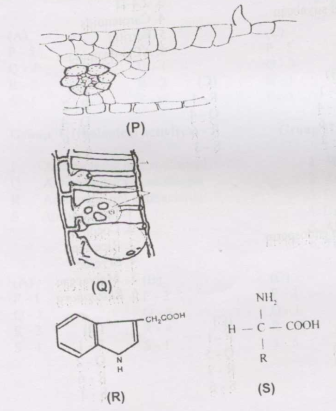
\includegraphics[width=0.5\columnwidth]{22match.png}
	\caption*{}
	\label{fig:Q22match}
	\end{figure}
		    \end{flushleft}
	    \begin{minipage}{0.5\columnwidth}
		    \begin{flushleft}
		    Group II
    \begin{enumerate}
        \item Amino acid
        \item Glucose
        \item IAA
        \item Bulliform cells
        \item Tyloses
        \item Kinetin
    \end{enumerate}
		    \end{flushleft}
	    \end{minipage}
    \begin{tabular}{l l l l}
     (A) & (B) & (C) & (D) \\
     P-5 & P-4 & P-5 & P-4 \\
     Q-2 & Q-6 & Q-4 & Q-5 \\
     R-3 & R-3 & R-6 & R-1 \\
     S-4 & S-1 & S-2 & S-2 \\
    \end{tabular}
\hfill{\textbf{GATE XL 2007}}
\section*{Common Data Questions}
\subsection*{Common Data for Questions 23, 24:}
A researcher studies three independently assorting genes in a plant. Each gene has a dominant and a recessive allele. The alleles are: $T$: tall plant; $t$: dwarf plant; $W$: purple flower; $w$: white flower; $C$: full pods; $c$: constricted pods. A cross was conducted between $TtWwCc \times TtwwCc$.

\vspace{1em} % Adds a small vertical space

\item How many different kinds of $F_1$ gametes would be expected from the above cross?
\begin{enumerate}
    \item 2
    \item 4
    \item 8
    \item 16
\end{enumerate}

\hfill{\textbf{GATE XL 2007}}
\item How many different kinds of $F_2$ genotypes would be expected from the above cross?
\begin{enumerate}
    \item 8
    \item 9
    \item 16
    \item 27
\end{enumerate}\hfill{\textbf{GATE XL 2007}}

\vspace{2em}

\section*{Linked Answer Questions}
\subsection*{Linked Answer Questions: Q. 25 to Q. 26 carry two marks each.}

\textbf{Statement for Linked Answer Questions 25 \& 26:}
Enzyme [E] reacts with substrate  to form an [ES] complex at normal temperature to produce the product. In the presence of inhibitor the rate of reaction changes.

\item Which of the following statements are \textbf{INCORRECT} about enzyme-mediated reaction in presence of inhibitor?
\begin{enumerate}
    \item Competitive inhibition causes rise in $K_m$ value without altering $V_{max}$.
    \item Noncompetitive inhibition causes decrease in $V_{max}$ and rise in $K_m$.
    \item Uncompetitive inhibition causes decrease in $V_{max}$ without altering $K_m$.
    \item Uncompetitive inhibition is rare and causes a decrease in both $V_{max}$ and $K_m$.
\end{enumerate}
\begin{enumerate}
    \item P, Q
    \item Q, R
    \item P, R
    \item P, S
\end{enumerate}\hfill{\textbf{GATE XL 2007}}

\item Identify the correct expression for noncompetitive and competitive inhibition.

\begin{table}[H]
	\begin{tabular}{|c|c|c|}
    \hline
     & Slope & Intercept on ordinate \\
    \hline                                                       
    P & $K_m/V_{max}(1+I/K_i)$ & $1/V_{max}(1+I/K_i)$ \\
    \hline
    Q & $K_m/V_{max}(1+I/K_i)$ & $1/V_{max}$ \\
    \hline
    R & $K_m/V_{max}$ & $1/V_{max}(1+I/K_i)$ \\
    \hline
    S & $K_m/V_{max}$ & $1/V_{max}$ \\
    \hline
\end{tabular}


	\caption*{}
	\label{26}
\end{table}
\vspace{1em}

	\begin{enumerate}
    \item P, S
    \item R, S
    \item P, Q
    \item Q, R
\end{enumerate}\hfill{\textbf{GATE XL 2007}}

\vspace{2em}

\section*{End of Section}
\subsection*{Statement for Linked Answer Questions 27 \& 28:}
Economically important plants are known for their commercial products and recognized with scientific names.

\item From the given common names, identify sequentially the scientific names of the following plants:
Common names: Cotton, Peanut, Sarpagandha and Tea
\begin{enumerate}
    \item P. \textit{Camelia sinensis}
    \item Q. \textit{Arachis hypogea}
    \item R. \textit{Rauwolfia serpentina}
    \item S. \textit{Gossypium arboreum}
\end{enumerate}
\begin{enumerate}
    \item P, Q, R, S
    \item S, R, Q, P
    \item S, Q, R, P
    \item S, P, R, Q
\end{enumerate}\hfill{\textbf{GATE XL 2007}}

\item Identify the most important commercial products from the above mentioned plants. (Follow the sequence of the common names)
    P. Vegetable Oil
    Q. Fibre
    R. Alkaloid
    S. Beverage
\begin{enumerate}
    \item Q, P, R, S
    \item S, Q, R, P
    \item C. Q, R, P, S
    \item D. R, Q, P, S
\end{enumerate}\hfill{\textbf{GATE XL 2007}}
\end{enumerate}

\begin{center}
\textbf{END OF THE SECTION}
\end{center}

\newpage

\section*{L: Microbiology}
\subsection*{Q.1-Q.6 carry one mark each.}
\section*{Q.1 - Q. 6 carry one mark each.}

\begin{enumerate}
\item Reverse transcriptase used in genetic engineering was discovered by
\begin{enumerate}
    \item Temin \& Baltimore
    \item Smith \& Arber
    \item Smith \& Baltimore
    \item Temin \& Arber
\end{enumerate}\hfill{\textbf{GATE XL 2007}}

\item Infection of $E.coli$ by bacteriophage is normally detected by
\begin{enumerate}
    \item Resistance of the bacteria to an antibiotic
    \item Growth of single colony on the agar plate
    \item The appearance of plaques or lysed bacteria on agar plates
    \item Restriction digest of the bacterial DNA
\end{enumerate}\hfill{\textbf{GATE XL 2007}}

\item A microscope that has a total magnification of 1500X with an oil immersion lens has an ocular of power
\begin{enumerate}
    \item 1.5X
    \item 15X
    \item 150X
    \item 1500X
\end{enumerate}\hfill{\textbf{GATE XL 2007}}

\item Which of the following species shows a high resistance to radiation damage?
\begin{enumerate}
    \item Deinococcus
    \item Micrococcus
    \item Staphylococcus
    \item Planococcus
\end{enumerate}\hfill{\textbf{GATE XL 2007}}

\item Peptic ulcers are caused by
\begin{enumerate}
    \item Shigella sonel
    \item Giardia lambas
    \item Enterobacter vermicularis
    \item Helicobacter pylori
\end{enumerate}\hfill{\textbf{GATE XL 2007}}

\item The evolutionary history of an organism is called
\begin{enumerate}
    \item Taxonomy
    \item Dendrogram
    \item Phylogeny
    \item Cladogram
\end{enumerate}\hfill{\textbf{GATE XL 2007}}

\vspace{2em}

\section*{Q.7 - Q. 24 carry two marks each.}

\item Which vector would be the most appropriate for cloning a 150 kb fragment of DNA?
\begin{enumerate}
    \item pBR322
    \item $\lambda$ vector
    \item YAC
    \item BAC
\end{enumerate}\hfill{\textbf{GATE XL 2007}}

\item Which group of microorganisms have a high level of unsaturated fatty acids in their cell membrane?
\begin{enumerate}
    \item Mesophilic
    \item Psychrophilic
    \item Thermophilic
    \item Hyperthermophilic
\end{enumerate}\hfill{\textbf{GATE XL 2007}}

\item Complete denitrification of nitrate results in the formation of
\begin{enumerate}
    \item N\textsubscript{2}
    \item NH\textsubscript{3}
    \item N\textsubscript{2}O
    \item NH\textsubscript{2}OH
\end{enumerate}\hfill{\textbf{GATE XL 2007}}

\item Which of the following disease is NOT caused by the Coxsackie virus?
\begin{enumerate}
    \item Intestinal infection
    \item Meningitis
    \item Gingivitis
    \item Myocarditis
\end{enumerate}\hfill{\textbf{GATE XL 2007}}

\item Bacterial cell wall biosynthesis is inhibited by the antibiotic
\begin{enumerate}
    \item Vancomycin
    \item Tetracycline
    \item Chloramphenicol
    \item Erythromycin
\end{enumerate}\hfill{\textbf{GATE XL 2007}}

\item Match the correct combination of plasmid DNA to their properties
\begin{enumerate}
    \item (P) Conjugative plasmid
    \item (Q) Cryptic plasmid
    \item (R) Episome
\end{enumerate}\hfill{\textbf{GATE XL 2007}}
\begin{enumerate}
    \item can integrate into the chromosome and replicate when the chromosome is copied
    \item capable of transferring itself between prokaryotes
    \item Does not appear to have any function
\end{enumerate}\hfill{\textbf{GATE XL 2007}}

\item An Hfr bacterium is one that contains
\begin{enumerate}
    \item Many unusual plasmids
    \item Chromosomal material acquired from a recipient cell
    \item The ability to undergo transduction
    \item A plasmid integrated into its chromosome
\end{enumerate}\hfill{\textbf{GATE XL 2007}}

\item Match the following product/process to the microorganism involved
\begin{enumerate}
    \item (P) Bioplastics
    \item (Q) Biofertilization
    \item (R) Biodegrading
    \item (S) Biopesticide
\end{enumerate}\hfill{\textbf{GATE XL 2007}}
\begin{enumerate}
    \item \textit{Beauveria bassiana}
    \item \textit{Azotobacter chroococcum}
    \item \textit{Ralstonia eutropha}
    \item \textit{Pseudomonas putida}
\end{enumerate}\hfill{\textbf{GATE XL 2007}}

\item Which of the following enzymes convert glucose-6-phosphate to 6-phosphoglucono-d-lactone in the Entner-Doudoroff pathway?
\begin{enumerate}
    \item Glucose-6-phosphate dehydrogenase
    \item Phosphoglucoseisomerase
    \item Phosphoglucomutase
    \item 6-phosphogluconate dehydratase
\end{enumerate}\hfill{\textbf{GATE XL 2007}}
\section*{} % This is an empty section header to match the formatting of the source image.

\item The process in which a molecule is transported into the cell while being chemically altered is called
\begin{enumerate}
    \item Passive transport
    \item Group translocation
    \item Facilitated transport
    \item None of the above
\end{enumerate}\hfill{\textbf{GATE XL 2007}}

\item MacConkey agar is a type of
\begin{enumerate}
    \item Selective media
    \item Differential media
    \item Both selective \& differential media
    \item None of these
\end{enumerate}\hfill{\textbf{GATE XL 2007}}

\item Which of the following modes of DNA replication are used by bacteria?
\begin{enumerate}
    \item Rolling circle
    \item Theta replication
    \item Bidirectional replication
    \item All of the above
\end{enumerate}\hfill{\textbf{GATE XL 2007}}

\item Which of the following is \textbf{INCORRECT} about negative staining procedure?
\begin{enumerate}
    \item It utilizes a stain such as Nigrosin
    \item Microorganisms stain deeply
    \item Microorganisms repel the dye
    \item An acidic dye is used
\end{enumerate}\hfill{\textbf{GATE XL 2007}}

\item A mutation in the codon UCG to UAG is described as
\begin{enumerate}
    \item Nonsense mutation
    \item Silent mutation
    \item Mis-sense mutation
    \item Neutral mutation
\end{enumerate}\hfill{\textbf{GATE XL 2007}}

\item The ineffectiveness of many antibiotics today is closely associated with
\begin{enumerate}
    \item Bacteriophages
    \item F plasmids
    \item R plasmids
    \item Bacterial transformations
\end{enumerate}\hfill{\textbf{GATE XL 2007}}

\item Which type of cells actually secrete antibodies?
\begin{enumerate}
    \item T cells
    \item Macrophages
    \item Monocytes
    \item Plasma cells
\end{enumerate}\hfill{\textbf{GATE XL 2007}}

\vspace{1em}
\section*{Common Data Questions}

\textbf{Common Data for Questions 23, 24:}
The 50$\mu$L of competent E.coli cells ($10^9$ CFU/mL) were transformed using 0.5$\mu$g of a 5kb plasmid DNA to which 950$\mu$L of SOC medium was added. Only 50 $\mu$L of this was plated on a selective agar plate. After an 12h incubation at 37\textdegree C, 90 colonies were observed.

\item Calculate the efficiency of this transformation in CFU/$\mu$g of DNA
\begin{enumerate}
    \item $3.6 \times 10^3$
    \item $3.6 \times 10^5$
    \item $1.8 \times 10^3$
    \item $1.8 \times 10^5$
\end{enumerate}\hfill{\textbf{GATE XL 2007}}

\vspace{2em}


\item Calculate the percentage of transformed cells
\begin{enumerate}
    \item 0.36\%
    \item 0.72\%
    \item 3.6\%
    \item 7.2\%
\end{enumerate}\hfill{\textbf{GATE XL 2007}}

\vspace{2em}
\section*{Linked Answer Questions}
\subsection*{Linked Answer Questions: Q. 25 to Q. 28 carry two marks each.}

\textbf{Statement for Linked Answer Questions 25 \& 26:}
An egg sandwich got contaminated with $10^5$ cells of a bacterium. It was left open at 37\textdegree C for 4 hours. It was found to contain 10000 cells.

\item What is the generation time of this bacterium?
\begin{enumerate}
    \item 15 min
    \item 20 min
    \item 25 min
    \item 30 min
\end{enumerate}\hfill{\textbf{GATE XL 2007}}

\item If the initial inoculum was only 1 cell, then after 10 hours what will be the number of cells?
\begin{enumerate}
    \item $2^8$
    \item $2^{24}$
    \item $2^{30}$
    \item $2^{40}$
\end{enumerate}\hfill{\textbf{GATE XL 2007}}

\vspace{2em}

\subsection*{Statement for Linked Answer Questions 27 \& 28:}
A researcher desires to clone a gene (1kb) of a microorganism. Its genome size is 1.5$\times$10\textsuperscript{3} kb. The average size of its library fragment is 5kb.

\item What is the ratio of genome size of the microorganism relative to average size of the fragment in the gene library?
\begin{enumerate}
    \item 3000
    \item 1500
    \item 4500
    \item None of these
\end{enumerate}\hfill{\textbf{GATE XL 2007}}

\item The genomic library was created in vectors that were transformed into bacterial cells. If there is a 95\% probability of the transformation, how many recombinant bacterial colonies will have to be screened to find this particular gene?
\begin{enumerate}
    \item 7000
    \item 8000
    \item 9000
    \item 10000
\end{enumerate}\hfill{\textbf{GATE XL 2007}}
\end{enumerate}

\begin{center}
\textbf{END OF THE SECTION}
\end{center}

\newpage

\section*{M: Zoology}
\subsection*{Q.1-Q.6 carry one mark each.}

\section*{Q.1 - Q. 6 carry one mark each.}

\begin{enumerate}
\item Sickle-cell anemia is caused by mutation in
\begin{enumerate}
    \item Haemoglobin A
    \item Haemoglobin B
    \item Haemoglobin F
    \item Haemoglobin S
\end{enumerate}\hfill{\textbf{GATE XL 2007}}

\item Each individual antigenic determinant of the variable region of the antibody is referred to as
\begin{enumerate}
    \item Paratope
    \item Epitope
    \item Agritope
    \item Idiotiope
\end{enumerate}\hfill{\textbf{GATE XL 2007}}

\item Which of the following non-covalent interactions is considered as strongest ?
\begin{enumerate}
    \item Hydrophobic interactions
    \item Ionic bonds
    \item Hydrogen bonds
    \item Van der waals forces
\end{enumerate}\hfill{\textbf{GATE XL 2007}}

\item Acrosome present on the sperm head is derived from
\begin{enumerate}
    \item Golgi apparatus
    \item Nucleus
    \item Endoplasmic reticulum
    \item Centrosome
\end{enumerate}\hfill{\textbf{GATE XL 2007}}

\item The first site of hematopoiesis in the mouse embryo is
\begin{enumerate}
    \item Liver
    \item Bone marrow
    \item Spleen
    \item Yolk sac
\end{enumerate}\hfill{\textbf{GATE XL 2007}}

\item Which of the following fish is considered to be a 'living fossil' ?
\begin{enumerate}
    \item Protopterus
    \item Lepidosiren
    \item Latimeria
    \item Neoceratodus
\end{enumerate}\hfill{\textbf{GATE XL 2007}}

\vspace{2em}

\section*{Q.7 - Q. 24 carry two marks each.}

\item Albinism is controlled by a recessive gene (c). From a marriage between a normal pigmented person carrying genotype Cc and albino cc, what is the chance that an albino child will be born?
\begin{enumerate}
    \item 1/2
    \item 1/4
    \item 3/4
    \item 3/8
\end{enumerate}\hfill{\textbf{GATE XL 2007}}

\item Many fishes are able to live outside water with the help of special air chambers above the gills. Which one of the following fish does not have same adaptation?
\begin{enumerate}
    \item Anabas
    \item Saccobranchus
    \item Gobiuis
    \item Clarias
\end{enumerate}\hfill{\textbf{GATE XL 2007}}

\item The air sac plays an important role in the aerial life of flying birds. Which of the following is not a function of the air sac?
\begin{enumerate}
    \item As a resonator
    \item As a balloon
    \item In perching
    \item Regulator of moisture content of the body
\end{enumerate}\hfill{\textbf{GATE XL 2007}}

\item Transgenic mice are produced by
\begin{enumerate}
    \item in vitro fertilization of ova by sperms from a different strain followed by implantation
    \item Transfer of cloned foreign DNA into blastocyst cells followed by implantation
    \item Implantation of cloned blastocyst cells from two different strains
    \item Selection of a given trait by repeated back-crossing
\end{enumerate}\hfill{\textbf{GATE XL 2007}}

\item Which of the following proteins binds tightly to DNA in the chromatin structure and influences eukaryotic DNA replication?
\begin{enumerate}
    \item Histones
    \item Lamina
    \item Vimentin
    \item Proteasome
\end{enumerate}\hfill{\textbf{GATE XL 2007}}

\item During DNA replication significant proportion of newly synthesized DNA in the lagging strand exists as small Okazaki fragments. The sizes of these units in bacteria are approximately
\begin{enumerate}
    \item 100 nucleotides
    \item 1000 nucleotides
    \item 100 base pairs
    \item 1000 base pairs
\end{enumerate}\hfill{\textbf{GATE XL 2007}}

\item Which of the following statement is not included in the inductions and deductions of Darwinism?
\begin{enumerate}
    \item The prodigality of reproduction is very important since over crowdedness results in struggle for existence
    \item In the struggle for existence the organisms with variation in structure habits or instincts may be better adapted to new conditions and will have better chance of survival
    \item Natural selection operates amongst the fittest and the new forms are established leading to speciation
    \item There is no organism without genotype. The genotype should be changed to give an efficient organism.
\end{enumerate}\hfill{\textbf{GATE XL 2007}}
\item In case of turtles, the temperature at which the eggs are exposed during development is the deciding factor in sex determination. This is because of the temperature sensitivity of
\begin{enumerate}
    \item Estrogen
    \item Testosterone
    \item Aromatase enzyme
    \item Progesterone
\end{enumerate}\hfill{\textbf{GATE XL 2007}}

\item One of the most remarkable features of evolution is the formation of the amnion and the allantoin, which appeared for the first time in
\begin{enumerate}
    \item Amphibians
    \item Fishes
    \item Birds
    \item Reptiles
\end{enumerate}\hfill{\textbf{GATE XL 2007}}

\item For cloning an animal, which of the following somatic cells would not be suitable?
\begin{enumerate}
    \item Lymphocytes
    \item Fibroblasts
    \item Epidermal cell
    \item Neuronal cell
\end{enumerate}\hfill{\textbf{GATE XL 2007}}

\item Differential blood cell counting is carried out routinely not only for assessing the "general health" of an individual but also for identifying types of infection. Increase in the circulatory eosinophils is likely to be due to infection with
\begin{enumerate}
    \item Viruses
    \item Helminths
    \item Fungi
    \item Bacteria
\end{enumerate}\hfill{\textbf{GATE XL 2007}}

\item Rajesh and Deb while playing in the field got stung by a comparable number of bees. After about 15 minutes, while Rajesh experienced acute pain and local swelling, Deb manifested intense swelling, breathlessness and had to be hospitalized. Which of the following reasons would be the most logical explanation for the different reactions?
\begin{enumerate}
    \item Deb was on an empty stomach
    \item Rajesh is several years younger than Deb
    \item Deb had been stung by bees before
    \item Deb is several years younger than Rajesh
\end{enumerate}\hfill{\textbf{GATE XL 2007}}

\item Normally receptors are cell-membrane bound but with few exceptions. Which of the following receptors is present in the cytoplasm?
\begin{enumerate}
    \item Thyroid stimulating hormone receptor
    \item Epidermal growth factor receptor
    \item Progesterone receptor
    \item Cytokine receptor
\end{enumerate}\hfill{\textbf{GATE XL 2007}}

\vspace{2em}

\item During development of the red blood cells from the stem cells of most mammals, the phenomenon of enucleation is observed during the last stage of differentiation. However, the red blood cells of some animals are nucleated: Identify which one of the following?
\begin{enumerate}
    \item Cow
    \item Rhinoceros
    \item Camel
    \item Polar bear
\end{enumerate}\hfill{\textbf{GATE XL 2007}}

\item Comparison of the genome sequences of any two animals would reveal evolutionary relatedness. In this context, the similarity between man and chimpanzee is
\begin{enumerate}
    \item $>$ 95\%
    \item $>$ 75\%
    \item $<$ 25\%
    \item $<$ 50\%
\end{enumerate}\hfill{\textbf{GATE XL 2007}}

\item Certain types of cancers can be correlated with specific changes in chromosome structure. In patients suffering from myelogenous leukemia, the abnormal chromosome detected was termed Philadelphia chromosome. Which of the following chromosome is altered in this disease?
\begin{enumerate}
    \item Chromosome 10
    \item Chromosome 11
    \item Chromosome 20
    \item Chromosome 22
\end{enumerate}\hfill{\textbf{GATE XL 2007}}

\vspace{2em}
\section*{Common Data Questions}
\textbf{Common Data for Questions 23, 24:}
The size of mammalian heart is nearly proportional to body size and makes up approximately 0.5\% of the body mass. However the heart rate is inversely related to body size. The following graph represents the relationship between the heart rate and body size of the mammals (data are plotted on logarithmic coordinates).
\begin{figure}[h!]
	\centering
	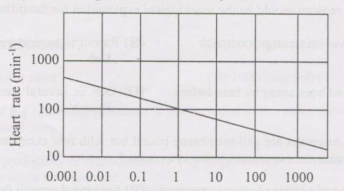
\includegraphics[width=\columnwidth]{23.png}
	\caption*{}
	\label{fig:Q23}
	\end{figure}

\item 1 kg bird is expected to have a heart of 8.2 g. For a mammal of the same size, the expected size of the heart could be
\begin{enumerate}
    \item 11.8 g
    \item 5.9 g
    \item 2.95 g
    \item 23.6 g
\end{enumerate}\hfill{\textbf{GATE XL 2007}}

\item An elephant that weights 3000 kg has a resting pulse rate of 25 per minute. What would be the possible range of the pulse rate of a 3 g shrew (the smallest living mammal)?
\begin{enumerate}
    \item 25
    \item 125
    \item 250
    \item Above 500
\end{enumerate}\hfill{\textbf{GATE XL 2007}}

\vspace{2em}

\section*{Linked Answer Questions: Q. 25 to Q. 28 carry two marks each.}

\subsection*{Statement for Linked Answer Questions 25 \& 26:}
An experiment was carried out to study the immune response to dust mite allergens in two strains of mice viz., BALB/c(b) and Nude(n). The mice were administered the immunogen on days 0 and 4 and allergen specific circulatory antibodies were monitored in the two groups of mice on days 7 and 14.

\item Which of the following class of antibodies would be detected in these strains of mice on day 7?
\begin{enumerate}
    \item IgM (b) IgM (n)
    \item IgG (b) IgM (n)
    \item IgA (b) IgM (n)
    \item IgE (b) IgM (n)
\end{enumerate}\hfill{\textbf{GATE XL 2007}}

\item Which of the following class of antibodies would be detected in the two strains of mice on day 14?
\begin{enumerate}
    \item IgG (b) IgM (n)
    \item IgE (b) IgE (n)
    \item IgE (b) IgM (n)
    \item IgG (b) IgG (n)
\end{enumerate}\hfill{\textbf{GATE XL 2007}}

\vspace{2em}

\subsection*{Statement for Linked Answer Questions 27 \& 28:}
A woman has a rare abnormality of the eye that has been found to be dependent on a single dominant gene (P). The woman's father had abnormal eyes but mother had normal eyes.

\item If the woman marries a man with normal eyes, what proportion of her children will have abnormal eyes?
\begin{enumerate}
    \item 25\%
    \item 50\%
    \item 75\%
    \item 100\%
\end{enumerate}\hfill{\textbf{GATE XL 2007}}

\item Which of the following representation does not explain the genotype of the woman's father?
\begin{enumerate}
    \item Heterozygous for P
    \item Homozygous for P
    \item Dominant for P
    \item Recessive for P
\end{enumerate}\hfill{\textbf{GATE XL 2007}}

\begin{center}
\textbf{END OF THE SECTION}
\end{center}
\end{enumerate}

\end{document}

